\chapter{Descrizione del contesto}
\label{sec:2_descrizione_contesto}

In questo capitolo saranno presentati diversi concetti di base che consentono una comprensione più completa dei capitoli successivi. Vengono in primo luogo introdotti i concetti di cloud computing ed edge computing, e di come abbiano portato alla nascita di nuovi paradigmi come ``Function as a Service'' e ``Decentralized FaaS''. A seguire, viene introdotto l'Apprendimento per Rinforzo, dettagliandone i concetti fondamentali e presentando l'approccio Deep Learning applicato all'apprendimento per rinforzo.

\section{Cloud computing}

In \cite{Europe2012} la Commissione Europea definisce in sintesi il cloud computing come un modello che consente l'archiviazione, l'elaborazione e l'uso dei dati su computer remoti tramite Internet. In letteratura esistono molte definizioni, una delle più conosciute e accettata è indicata dal National Institute for Standards and Technology degli Stati Uniti (NIST) in \cite{Nist2011}, in cui il cloud computing viene descritto come un modello che consente un accesso onnipresente, conveniente e su richiesta a un insieme condiviso di risorse computazionali (reti, server, spazio di archivio, servizi...) che vengono rilasciate con uno sforzo minimo in termini di gestione o di interazione con i fornitori di servizi. Il NIST identifica alcune caratteristiche essenziali del modello: (1) self-service su richiesta, in cui il consumatore dispone di risorse computazionali senza l'intervento di un operatore umano; (2) accesso alla rete allargato per comprendere dispositivi eterogenei (computer, dispositivi mobili, sensori IoT); (4) visione delle risorse computazionali come un insieme in cui il consumatore ha solo una visione ad alto livello (per esempio, la posizione geografica della risorsa ma non il numero di server fisici); (4) elasticità rapida e automatica nella fornitura delle risorse per rispondere a carichi diversi, (5) misurazione del servizio per ottimizzare l'allocazione e il controllo delle risorse, oltre che per la tariffazione.

Nonostante il modello sia diventato popolare dagli anni 2010, il lancio di Amazon Web Services (AWS), Google Cloud Platform e Microsoft Azure, tra le principali piattaforme di cloud computing, è avvenuto tra il 2006 e il 2008  \cite{Amazon2006, McDonald2008, Roosevelt2022}. Tali piattaforme sono definite come ``cloud pubblico'' e sono una delle modalità previste per il deploy, insieme al cloud privato, ibrido o comunitario \cite{Nist2011}. In linea generale, la nascita del modello ha permesso la creazione di alternative alle infrastrutture on-premise\footnote{Software installato ed eseguito su risorse computazioni appartenenti al consumatore.}, consentendo agli utenti di delegare alle infrastrutture cloud la gestione delle risorse computazionali.

Anche se ogni piattaforma eroga servizi a livelli di astrazione diversi e non sempre comparabili tra di loro, il NIST ha identificato tre modelli di servizio fondamentali incrementali, illustrati anche in \Cref{fig:2_cloud_level_services}:

\begin{itemize}
    \item Infrastructure as a Service (IaaS): il consumatore può allocare determinate risorse computazionali ed eseguire software arbitrario, tra cui il sistema operativo, senza però controllare o gestire l'infrastruttura sottostante.

    \item Platform as a Service (PaaS): il consumatore può rilasciare applicazioni realizzate con linguaggi di programmazione, librerie, servizi e strumenti supportati dalle piattaforme, senza occuparsi della gestione dell'esecuzione delle applicazioni e dell'infrastruttura sottostante.
    
    \item Software as a Service (SaaS): il consumatore può soltanto utilizzare le applicazioni erogate e gestite dalla piattaforma senza poter controllare o gestire l'infrastruttura sottostante.
\end{itemize}

\begin{figure}
    \centering
    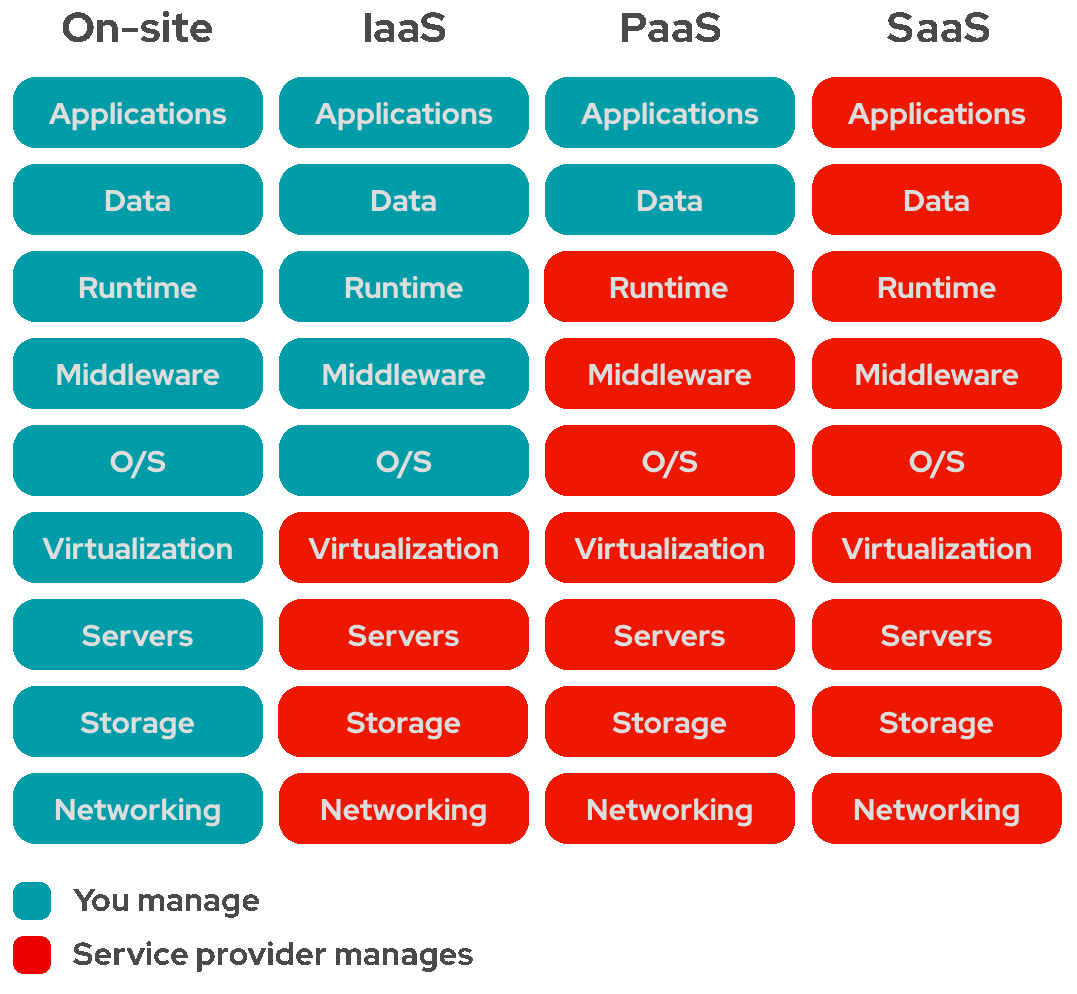
\includegraphics[width=.6\linewidth]{assets/2/cloud_level_services.png}
    \caption[Modelli di servizio fondamentali del cloud computing.]{Modelli di servizio fondamentali del cloud computing. Fonte: \url{https://www.redhat.com/en/topics/cloud-computing/iaas-vs-paas-vs-saas}}
    \label{fig:2_cloud_level_services}
\end{figure}

\subsection{Function as a Service}

Dalla nascita del cloud computing si sono evoluti nuovi paradigmi basati su esso, tra cui il serverless computing, definito in \cite{Castro2019} come una piattaforma che nasconde l'utilizzo del server agli sviluppatori ed esegue codice su richiesta in maniera automatica, scalabile e fatturata solo per il tempo effettivo di esecuzione. All'interno di questo modello sono presentati due approcci: Backend as a Service (BaaS), in cui la piattaforma eroga servizi di base, come la gestione dei database o dell'autenticazione, esponendo delle API che gli sviluppatori integrano per costruire le applicazioni; e Function as a Service (FaaS), di principale interesse per lo studio presentato in questa tesi.

L'approccio FaaS consente agli sviluppatori la creazione di applicazioni come insieme di funzioni, senza dover gestire l'infrastruttura necessaria per la loro esecuzione. Ogni funzione è specializzata un compito specifico ed è considerata come l'unita minima di esecuzione. L'infrastruttura FaaS è costituita da un modello di esecuzione ad eventi, in cui le funzioni sono:

\begin{itemize}
    \item Senza stato (stateless), per cui non viene mantenuta alcuna informazione con le esecuzioni precedenti,

    \item Temporanee, poiché le funzioni solo le risorse computazionali solo durante la loro esecuzione,

    \item Invocate da eventi, e quindi senza un processo costantemente attivo in attesa,

    \item Gestite dalla piattaforma, in cui lo sviluppatore è tariffato solo per le risorse utilizzate e le invocazioni.
\end{itemize}

Poiché le funzioni sono senza stato e basate su eventi, risultano facilmente scalabili in tempo reale in base al numero di richieste, poiché la piattaforma crea (o distrugge) delle copie in parallelo che si adattano per soddisfare la domanda.

La natura serverless di FaaS presenta vantaggi e svantaggi. Se FaaS permette a sviluppatori di accelerare lo sviluppo e alleggerire la gestione dell'infrastruttura, il modello non è pensato per l'esecuzione di funzioni per un lungo periodo di tempo. Inoltre FaaS soffre del problema ``cold start'': nel momento in cui una funzione viene invocata infatti, la piattaforma verifica la presenza di un’istanza pronta per eseguirla, ma nel caso in cui non esistesse allora ne viene avviata una nuova e ciò causa un aumento dei tempi di risposta, causando potenziali disagi agli applicativi che richiedono latenze contenute \cite{Ana2024}.

Ogni grande piattaforma di cloud computing offre un servizio FaaS, come Microsoft Azure Functions\footnote{\url{https://azure.microsoft.com/it-it/products/functions/}} o AWS Lambda\footnote{\url{https://aws.amazon.com/it/lambda/}}. Esistono inoltre implementazioni open source del modello FaaS, come Fission\footnote{\url{https://fission.io/}} e OpenFaaS\footnote{\url{https://www.openfaas.com/}}, di cui \Cref{fig:2_openfaas} ne mostra l'architettura dal punto di vista del gestore della piattaforma.

\begin{figure}
    \centering
    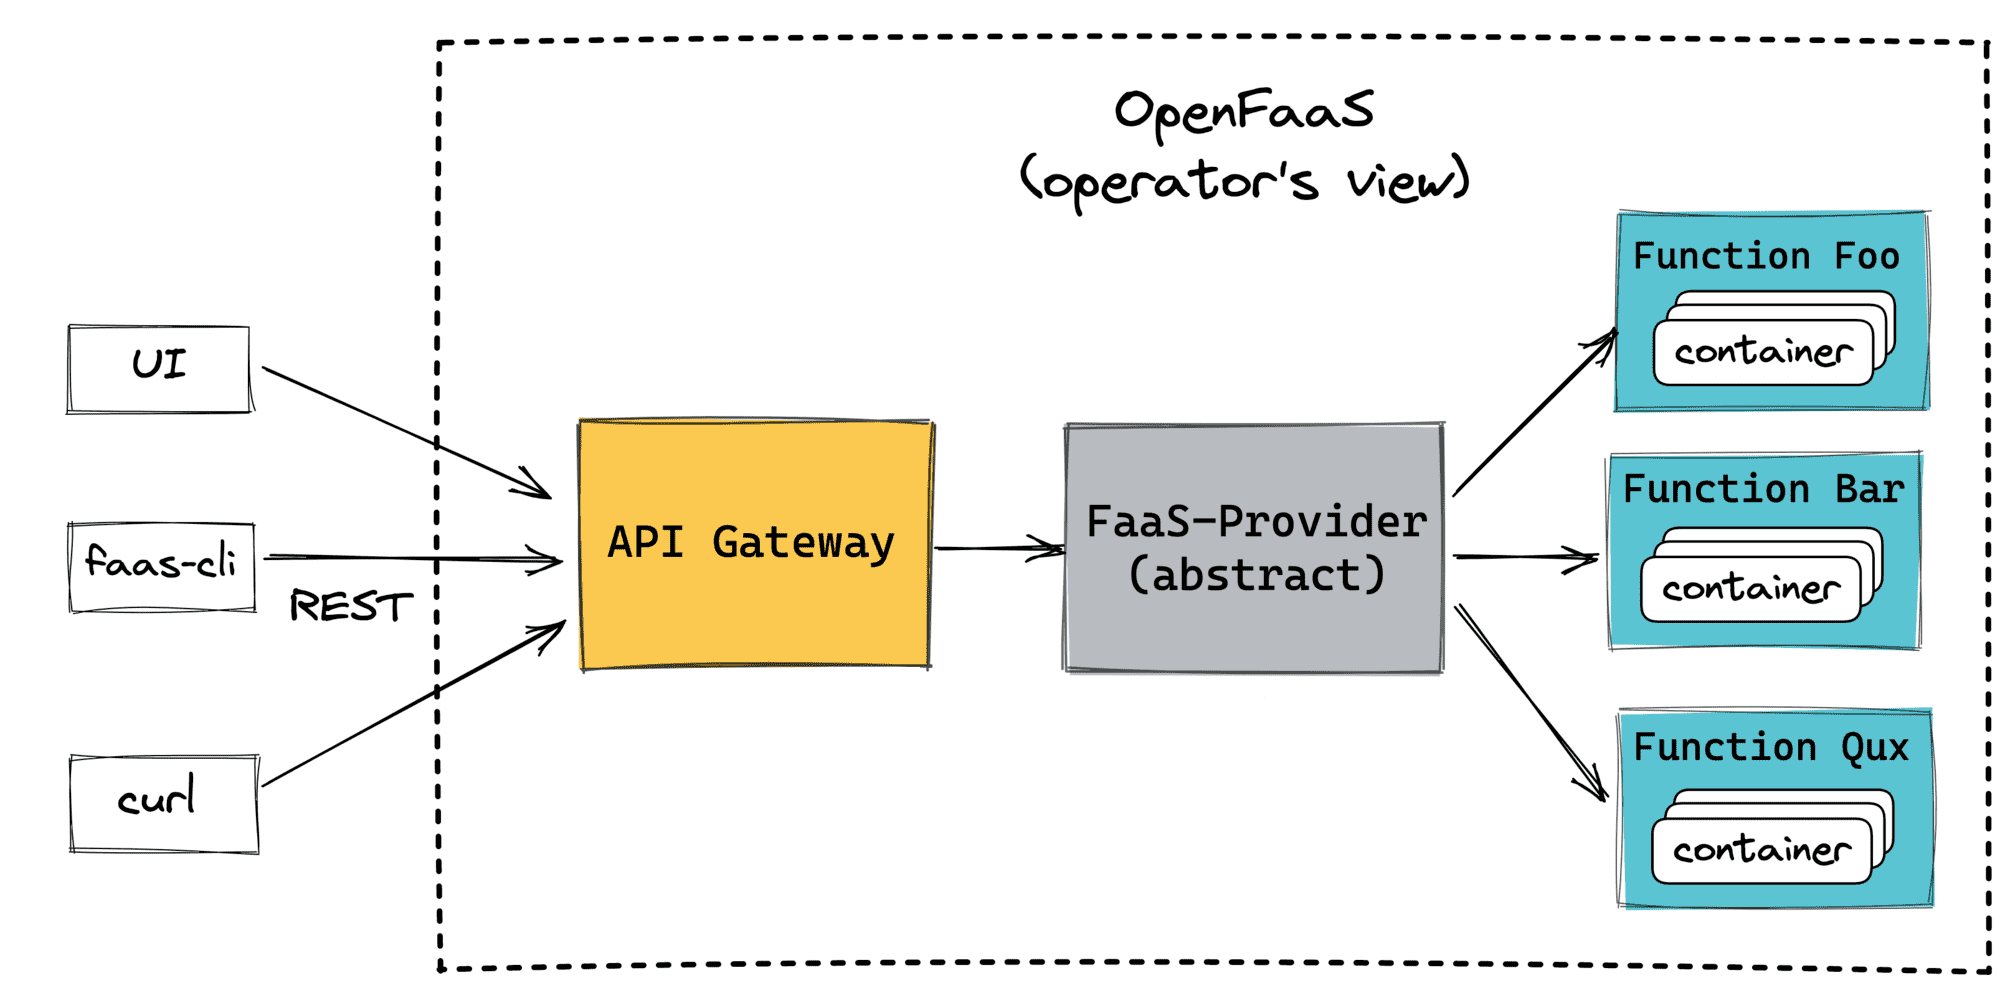
\includegraphics[width=0.8\linewidth]{assets/2/openfaas.png}
    \caption[Architettura generale di una piattaforma FaaS]{Architettura generale una piattaforma FaaS, nello specifico OpenFaaS. Fonte: \url{https://iximiuz.com/en/posts/openfaas-case-study/}}
    \label{fig:2_openfaas}
\end{figure}

\subsection{Edge computing}

Negli ultimi anni, il mondo dell'Internet of Things (IoT) ha vissuto uno sviluppo senza precedenti, con un aumento dei dispositivi e di connessioni che ha comportato una grande crescita nella produzione di dati, come si evince in \cite{Duarte2024}. L'analisi di questi dati può rivelarsi uno strumento importante, ma richiede una grande capacità computazionale in un unico preciso punto della rete. Sebbene il cloud computing possa essere utilizzato per questi scopi, ci sono delle limitazioni sulla possibilità di elaborare una tale quantità di dati, soprattutto se bisogna soddisfare richieste di utenti in termini di Qualità del Servizio (QoS), come esplicitato in \cite{Laroui2021}.

Per far fronte a queste necessità sono nati nuovi paradigmi denominati fog ed edge computing, presentati in modo più approfondito in \cite{Hurbungs2021}, il cui obiettivo principale è quello di spostare la computazione dal centro ai margini della rete. I vantaggi sono molteplici: consente di ridurre la latenza rispetto alla computazione presente al centro della rete, oltre a poter progettare una computazione suddivisa sui diversi livelli: le informazioni di minor valore possono infatti essere individuate e scartate ai bordi della rete, mentre i dati più importanti possono essere inoltrati al cloud per l’elaborazione definitiva. Si possono gestire all'edge dati che non possono essere mandati al cloud per questione di privacy, oppure perché sono richieste analisi in tempo reale che non sono compatibili con i ritardi che verrebbero introdotti con il cloud.

Se nel fog computing avviene la decentralizzazione di un’infrastruttura di elaborazione tramite ampliamento del cloud, attraverso il posizionamento strategico di nodi tra il cloud e i dispositivi terminali, nell'edge computing questo processo è portato all'estremo. Nell'edge computing la computazione è situata nei nodi periferici della rete, risultando, di conseguenza, più prossima all'utente finale e al luogo di generazione dei dati. La \Cref{fig:2_cloud_fog_edge} mostra la differenza dei tre modelli.

\begin{figure}
    \centering
    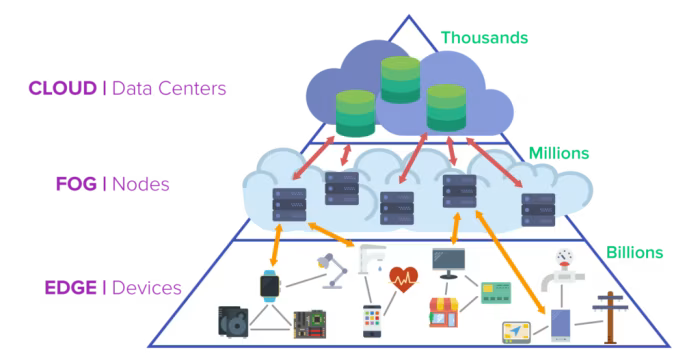
\includegraphics[width=.8\linewidth]{assets/2/cloud_fog_edge.png}
    \caption[Differenze tra cloud, fog ed edge computing]{Differenze tra cloud, fog ed edge computing. Fonte: \url{https://www.pubnub.com/blog/extending-cloud-technologies-to-the-edge/}}
    \label{fig:2_cloud_fog_edge}
\end{figure}

L'edge computing presenta diversi vantaggi: una minore latenza e maggiore velocità, dovuti dalla prossimità della computazione all'utente, riduzione dei costi ottimizzando il flusso dei dati verso i sistemi centrali, e infine una maggiore privacy e affidabilità, per via dell'elaborazione in loco.

\subsection{Decentralized FaaS}
\label{sec:2_dfaas}

Il paradigma FaaS convenzionale non è applicabile in un ambiente di edge computing, a causa del traffico dinamico e delle risorse computazionali limitate presenti sui nodi edge. Per poter mantenere i vantaggi di FaaS in tale ambiente è necessario quindi federare i nodi in ambienti di esecuzione distribuiti per bilanciare il carico tra di essi mediante la realizzazione di appositi algoritmi. Decentralized FaaS (DFaaS), introdotto in \cite{Ciavotta2021}, rappresenta proprio questo punto di unione tra i due modelli: l'architettura prevede degli ambienti federati e centralizzati in cui i nodi edge bilanciano automaticamente il traffico tra i nodi appartenenti a ecosistemi FaaS edge federati.

DFaaS utilizza una rete peer-to-peer overlay per scambiare dati sulla struttura della rete, tempi di risposta e capacità di carico dei nodi. Con l’espressione peer-to-peer si intende una rete formata da nodi connessi tra loro, che non hanno una gerarchia, ma sono equipotenti, o peer (pari). In linea generale, all'interno di questa architettura i nodi sovraccarichi utilizzano le informazioni scambiate nella rete per indirizzare alcune delle richieste di esecuzione FaaS ai nodi meno congestionati.

Lo scenario di riferimento di DFaaS, mostrato in \Cref{fig:2_dfaas_scenario}, consiste in una rete di nodi FaaS posti ai margini della rete e geograficamente distribuiti. In ciascun nodo è situata una piattaforma FaaS che esegue le funzioni serverless, tipicamente sotto forma di richieste HTTP, e per ciascun nodo è associato un punto di accesso per la connessione di rete. Di solito, uno o più nodi edge vengono gestiti da un edge provider, che potrebbe essere, ad esempio, un operatore di rete. I nodi possono appartenere al medesimo fornitore o a fornitori diversi e sono interconnessi tramite connessioni di rete, spesso regolate da accordi di livello di servizio (Service Level Agreement, SLA). L’ambiente descritto rappresenta un ecosistema federato di edge computing, in cui edge provider diversi, ciascuno con la propria piattaforma DFaaS e tecnologie specifiche, si uniscono in federazione. Così facendo, possono sfruttare in modo trasparente le risorse computazionali offerte dai nodi edge di altri fornitori. Questa collaborazione diventa particolarmente rilevante quando i nodi sperimentano un sovraccarico dovuto a picchi di traffico. 

\begin{figure}
    \centering
    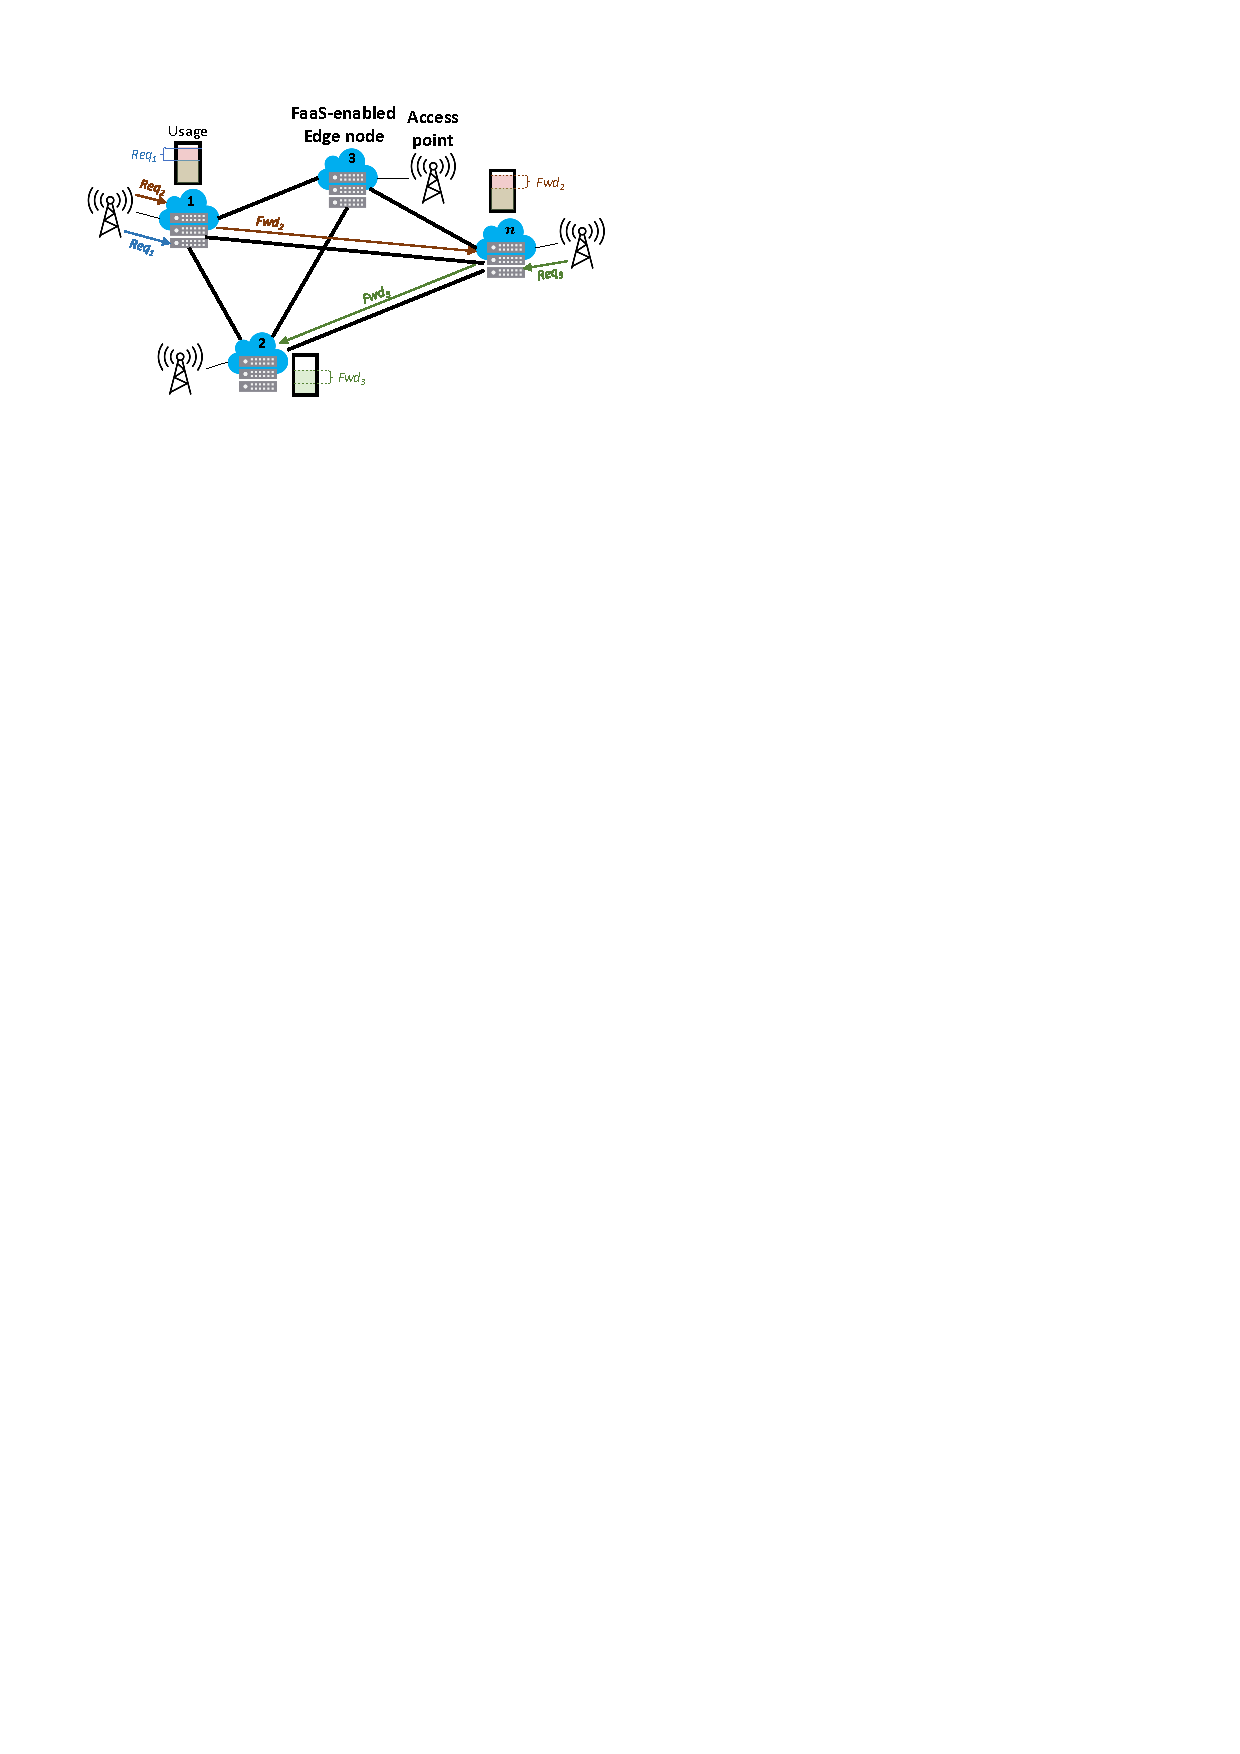
\includegraphics[width=.7\linewidth]{assets/2/dfaas_scenario.pdf}
    \caption[Scenario di riferimento di DFaaS]{Scenario di riferimento di DFaaS in \cite{Ciavotta2021}}
    \label{fig:2_dfaas_scenario}
\end{figure}

L'architettura di DFaaS è mostrata in \Cref{fig:2_dfaas_architecture}: si avvale di componenti consolidate, attivamente mantenute e testate, ponendo un'enfasi particolare sulla modularità, manutenibilità ed evolvibilità della piattaforma.

\begin{figure}
    \centering
    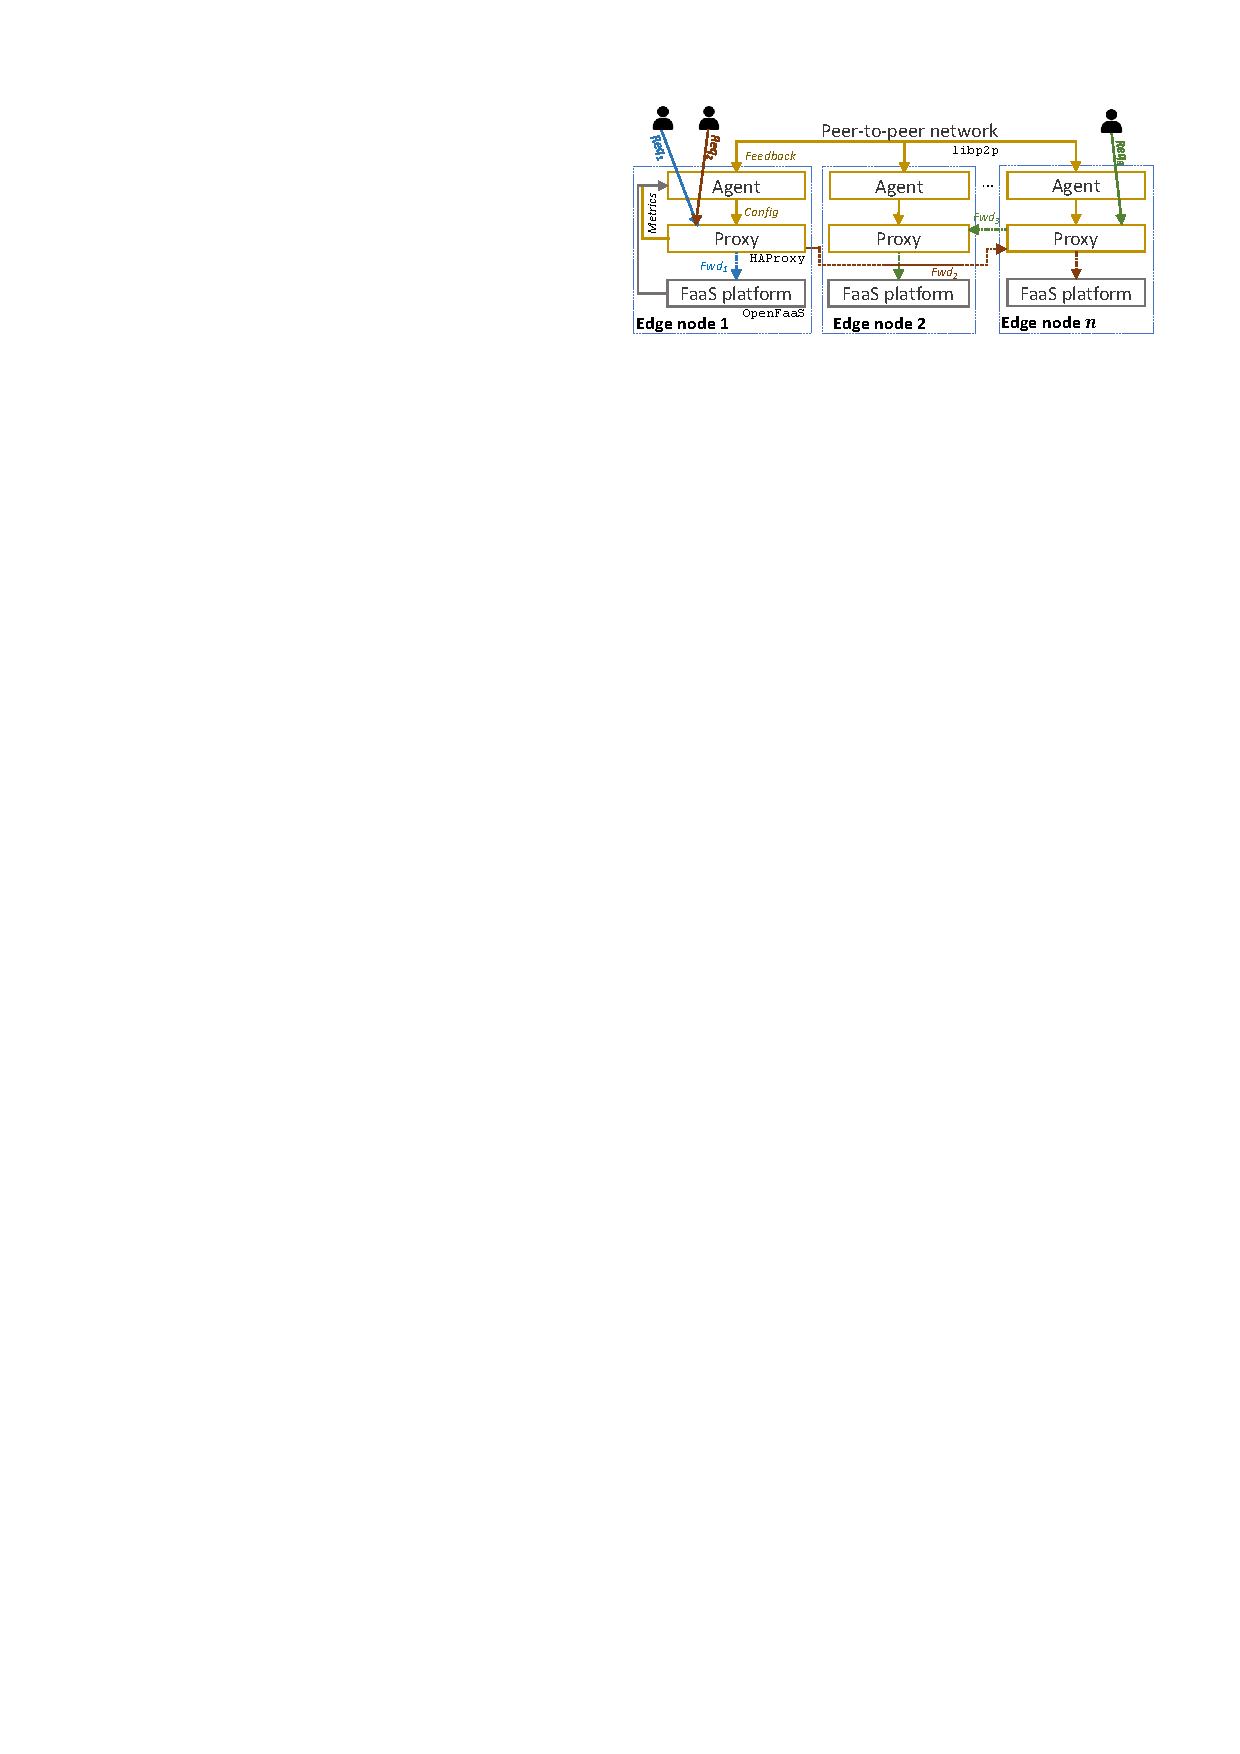
\includegraphics[width=.7\linewidth]{assets/2/dfaas_architecture.pdf}
    \caption[Architettura di DFaaS]{Architettura di DFaaS in \cite{Ciavotta2021}}
    \label{fig:2_dfaas_architecture}
\end{figure}

I principali componenti, replicati su tutti i nodi, sono:

\begin{itemize}
    \item Agenti: ogni agente è responsabile di gestire la connessione alla rete peer-to-peer e la comunicazione con gli altri agenti. Monitora periodicamente lo stato della piattaforma FaaS sul nodo in cui si trova, raccogliendo metriche pertinenti alle capacità computazionali disponibili. Configura il proxy per fare in modo di reindirizzare il traffico ai nodi previsti in base agli accordi che può negoziare con gli altri agenti. 

    \item Proxy: si occupa di gestire le richieste HTTP in ingresso, inoltrandole alla piattaforma FaaS locale oppure a un altro nodo edge. In DFaaS è implementato attraverso HAProxy\footnote{\url{https://www.haproxy.org/}}.  

    \item Piattaforma FaaS: si occupa di eseguire sul nodo locale la funzione invocata, allocando le risorse computazionali necessarie. DFaaS utilizza OpenFaaS.
\end{itemize}

Tale modello è stato considerato come l'obiettivo da replicare nello studio in questione, ponendo alcune semplificazioni per realizzare un ambiente simulato che tuttavia rispecchi gli aspetti caratteristici di DFaaS. Nel \Cref{sec:4_modellazione} verrà presentata la modellazione di DFaaS.

\section{Apprendimento per Rinforzo}

L'Apprendimento per Rinforzo (Reinforcement Learning, abbreviato RL) è un'area interdisciplinare del machine learning e del controllo che riguarda l'adattamento e l'ottimizzazione del comportamento di un agente all'interno di un ambiente dinamico, al fine di massimizzare una ricompensa cumulativa \cite{Sutton2018}. I componenti fondamentali in un sistema di RL sono i seguenti, mostrati anche in \Cref{fig:2_rl_components}:

\begin{itemize}
    \item Agente: è l'entità che sceglie le azioni,

    \item Ambiente: è il contesto in cui l'agente interagisce e su cui hanno effetto le azioni intraprese,

    \item Ricompensa: è un segnale numerico che quantifica la qualità di un'azione, allo scopo di incoraggiare la scelta di azioni corrette.
\end{itemize}

\begin{figure}
    \centering
    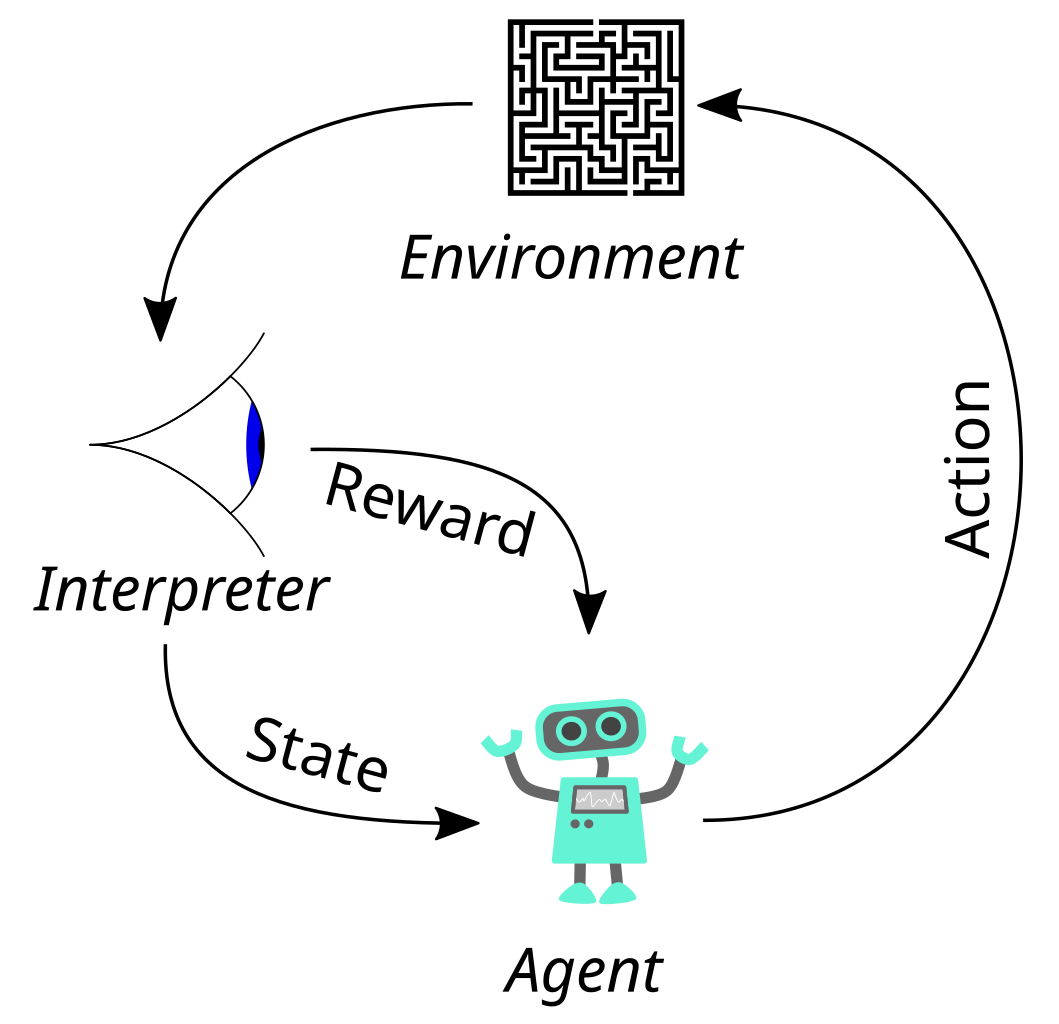
\includegraphics[width=.5\linewidth]{assets/2/rl_components.png}
    \caption[Componenti tipici in un sistema RL]{Componenti tipici in un sistema RL. Un agente prende decisioni in base all'osservazione (lo stato), tale azione produce delle conseguenze sull'ambiente che sono valutate e viene restituito il feedback all'agente, insieme al nuovo stato. Fonte: Megajuice, CC0, Wikimedia Commons.}
    \label{fig:2_rl_components}
\end{figure}

Un aspetto importante di un sistema RL è che all'agente non viene indicato quale azione deve intraprendere, bensì è l'agente stesso a scoprire in autonomia come agire per massimizzare la ricompensa sul lungo periodo. Nei casi più interessanti e complessi, le azioni possono influenzare non solo la ricompensa immediata, ma anche gli stati futuri del sistema e, attraverso questi, le ricompense future. L'apprendimento per tentativi ed errori e la ricompensa ritardata sono tra le due caratteristiche distintive dell'apprendimento per rinforzo. 

Un problema RL viene formalizzato come un un processo decisionale di Markov, approfondito nella \Cref{sec:2_mdp}, con l'obiettivo di trovare una policy\footnote{Una strategia che l'agente segue, definita nella \Cref{sec:2_rl_functions}.} ottimale per il processo, senza che l'agente sia a conoscenza dell'evoluzione del processo e di come vengono calcolate le ricompense. Tali processi possono essere risolti utilizzando algoritmi di programmazione dinamica\footnote{Tecnica in cui si semplifica un problema in sotto-problemi più semplici in modo ricorsivo.}. Tuttavia, questi richiedono di sviluppare un modello, con le difficoltà associate. Gli algoritmi RL invece non ipotizzano di conoscere esattamente il modello matematico, e possono quindi essere usati con modelli di grandi dimensioni che altrimenti sarebbero intrattabili con i metodi classici.

Un punto importante degli algoritmi RL è trovare un bilanciamento tra l'esplorazione (di un territorio inesplorato) e lo sfruttamento (dell'esperienza accumulata) con l'obiettivo di massimizzare la ricompensa nel lungo periodo, poiché  in cui il riscontro delle scelte può essere incompleto o ritardato. Il bilanciamento è importante perché un'eccessiva esplorazione può portare a perdere opportunità di ottenere ricompensa da azioni note, mentre un eccessivo sfruttamento può impedire all'agente la scoperta di nuove azioni più fruttuose.

\paragraph{Differenze tra RL e altri metodi.} Il RL si differenzia dall'apprendimento supervisionato, poiché RL non richiede un insieme di esempi etichettati ed è in grado di apprendere in contesti dinamici. Un'altra differenza riguarda la sparsità del feedback: il feedback che riceve un agente può non essere informativo finché l'ambiente non raggiunge un determinato stato. Infine c'è una differenza anche nella generazione dei dati, in cui nell'apprendimento supervisionato avviene in modo indipendente dall'algoritmo, mentre nel RL viene generato dall'agente che interagisce con l'ambiente.

Il RL si differenzia anche dall'apprendimento non supervisionato, perché ha come obiettivo la massimizzazione della ricompensa nel lungo periodo e non l'identificazione di strutture nascoste nei dati. Per questi motivi il RL è considerato come un paradigma a sé stante nel campo del machine learning.

\paragraph{} Di seguito verranno introdotti alcuni concetti essenziali del RL per comprendere al meglio le scelte e le tecniche usate per modellazione e applicazione di algoritmi del caso di studio. Per un quadro d'insieme introduttivo più ampio è possibile consultare \cite{Ghasemi2024}.

\subsection{Processo decisionale di Markov}
\label{sec:2_mdp}

Un processo decisionale di Markov (Markon Decision Process, MDP) è un modello decisionale che opera in modo sequenziale, con tempi definiti in passi discreti \cite{Puterman1994}. Un MDP è definito come una quadrupla $(\mathcal{S}, \mathcal{A}, \mathcal{P}, \mathcal{R})$:

\begin{itemize}
    \item $\mathcal{S}$ è l'insieme finito degli stati,

    \item $\mathcal{A}$ è l'insieme finito delle azioni,

    \item $\mathcal{P}$ è la funzione di probabilità di transizione tra gli stati, definita come ${\mathcal{P}: \mathcal{S} \times \mathcal{A} \times \mathcal{S} \to [0, 1]}$ per cui

    \begin{equation}
        \forall s \in \mathcal{S}, a \in \mathcal{A}: \sum_{s' \in \mathcal{S}} \mathcal{P}(s, a, s') = 1,
    \end{equation}

    \item $\mathcal{R}$ è la funzione di ricompensa, definita come $\mathcal{R}: \mathcal{S} \times \mathcal{A} \times \mathcal{S} \to \mathbb{R}$.
\end{itemize}

È importante sottolineare che gli agenti non hanno conoscenza delle funzioni di transizione $\mathcal{P}$ e di ricompensa $\mathcal{R}$, ma solo degli spazi delle azioni $\mathcal{A}$ e degli stati $\mathcal{S}$.

L'interazione tra l'agente e l'MDP produce una sequenza di esperienze, chiamata traiettoria e indicata come $\tau$, contenente la sequenza temporale di stati, azioni e ricompense incontrate dall'agente. La singola esperienza al passo $t$ è definita come una quadrupla $(s_t, a_t, r_t, s_{t+1})$, in cui

\begin{itemize}
    \item $s_t \in \mathcal{S}$ è lo stato dell'ambiente al passo $t$,

    \item $a_t \in \mathcal{A}$ è l'azione scelta dall'agente al passo $t$,

    \item $s_{t+1} \in \mathcal{S}$ è lo stato in cui l'ambiente si muove a seguito dell'azione $a_t$, scelta nello stato $s_t$ al passo $t$,

    \item $r_t = \mathcal{R}(s_t, a_t, s_{t+1})$ è la ricompensa ottenuta al passo $t$. \label{sec:2_reward_function_def}
\end{itemize}

Un esempio di MDP è mostrato in \Cref{fig:2_rl_mdp_example}.

\begin{figure}
    \centering
    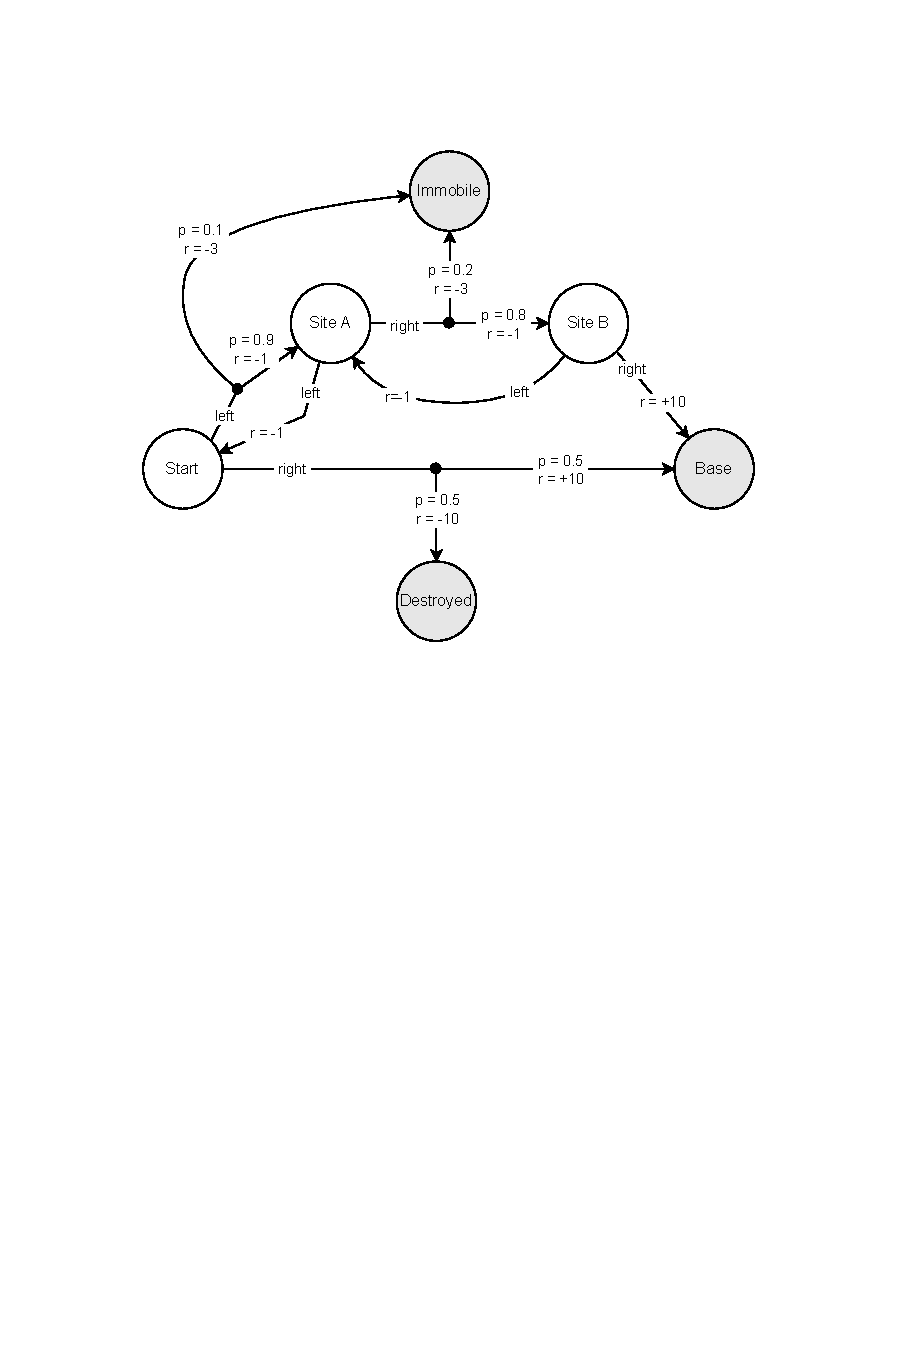
\includegraphics[width=.6\linewidth]{assets/2/rl_mdp_example.pdf}
    \caption[Esempio di un processo decisionale di Markov]{Esempio di un processo decisionale di Markov che modella il movimento di un rover su Marte. I cerchi sono gli stati, di cui quelli scuri sono terminali. A ogni stato sono associate due possibili azioni, destra e sinistra, mostrati come archi con la probabilità di transizione associata e la ricompensa. Fonte: \cite{Stefano2024}}
    \label{fig:2_rl_mdp_example}
\end{figure}

\paragraph{Proprietà di Markov.} Un MDP soddisfa la proprietà di Markov, da cui viene il nome: dato lo stato e la ricompensa attuale, lo stato e la ricompensa futuri non sono condizionati dagli stati e azioni passate, cioè:

\begin{equation}
    \mathbb{P}(s_{t+1}, r_t | s_t, a_t, s_{t-1}, \dots, s_0, a_0) = \mathbb{P}(s_{t+1}, r_t | s_t, a_t).
\end{equation}

Ne consegue che lo stato corrente fornisce le informazioni sufficienti per scegliere un'azione ottimale in un MDP, e che gli stati e azioni del passato non sono rilevanti.

\paragraph{Guadagno atteso scontato.} Data una traiettoria, il guadagno è la somma delle ricompense ottenute. Per via della natura stocastica di un MDP, non è possibile per l'agente massimizzare il guadagno per tutte le traiettorie, bensì l'obiettivo dell'agente è massimizzare il guadagno atteso per qualsiasi traiettoria, definito come:

\begin{equation}\label{eq:2_discounted_return}
    \mathbb{E} \left[ r_0 + \gamma r_1 + \gamma^2 r_2 + \dots \right] = \mathbb{E} \left[ \sum_{t=0}^{\infty} \gamma^t r_t \right].
\end{equation}

Poiché una traiettoria può essere infinita, per ottenere un valore atteso finito viene introdotto il fattore di sconto $\gamma \in [0, 1]$. Con un valore vicino a 0 le ricompense future avranno poca importanza, mentre vicino a 1 saranno considerate rilevanti. L'\Cref{eq:2_discounted_return} viene chiamata \textit{guadagno atteso scontato}.

\paragraph{MDP episodici e continui.} Una traiettoria in un MDP come presentato è infinita, poiché non esiste il concetto di stato terminale. MDP di questa tipologia si chiamano \textit{continui} o \textit{non-episodici}. Nonostante esistano definizioni di modelli più avanzati di MDP che introducono stati terminali, si può realizzare lo stesso concetto con un MDP: uno stato che una volta raggiunto rimane nello stesso stato, qualsiasi sia l'azione scelta dall'agente. Questa tipologia di MDP si chiama \textit{episodica}, perché ha una durata limitata di numero di interazioni, o \textit{passi}.

\subsection{Funzioni fondamentali}
\label{sec:2_rl_functions}

In un sistema di RL l'obiettivo dell'agente è massimizzare il guadagno atteso scontato. Per raggiungere questo scopo, l'agente può imparare una delle tre funzioni primarie:

\begin{itemize}
    \item Policy: è la strategia che l'agente segue per prendere una decisione a partire da uno stato. Una policy $\pi$ è tipicamente stocastica, pertanto è definita come

    \begin{equation}
        \pi: \mathcal{A} \times \mathcal{S} \to [0, 1], \qquad \pi(a, s) \coloneqq \mathbb{P}(a_t = a | s_t = s)
    \end{equation}
    
    e si indica come $a \sim \pi(s)$ l'azione $a$ estratta dalla policy $\pi$ per lo stato $s$.
    
    La policy $\pi$ esprime quindi la probabilità di scegliere un'azione a partire da uno stato, e può essere rappresentata mediante una funzione, una tabella o, in scenari più complessi, attraverso modelli stocastici o reti neurali.
    
    Esistono anche policy deterministiche, in cui dato uno stato viene scelta sempre la stessa azione, ma sono meno comunemente applicate rispetto alle policy stocastiche perché quest'ultime si adattano in scenari con una grande varianza nelle dinamiche di transizione.

    \item Funzione di valore e valore-azione: sono due funzioni strettamente collegate, in cui

    \begin{itemize}
        \item Funzione di valore: quantifica il guadagno atteso a partire da uno stato $s$, ipotizzando che l'agente continui a operare con la stessa policy $\pi$. Rappresentata in letteratura come $V^\pi$, è definita come:

        \begin{equation}
            V^\pi: \mathcal{S} \to \mathbb{R}, \qquad V^\pi(s) \coloneqq \mathbb{E}_{s_0=s, \tau \sim \pi} \left[ \sum_{t=0}^{\infty} \gamma^t r_t\right].
        \end{equation}
    
        Questo concetto permette di valutare l’efficacia di una sequenza di azioni nel lungo termine, anche quando alcune di queste possono sembrare inizialmente sconvenienti.

        \item Funzione Valore-Azione: quantifica il guadagno atteso scegliendo un'azione $a$ da uno stato $s$, ipotizzando che l'agente continui in seguito a operare con la stessa policy $\pi$. Rappresentata in letteratura come $Q^\pi$, è definita come

        \begin{equation}
            Q^\pi: \mathcal{S} \times \mathcal{A} \to \mathbb{R}, \qquad Q^\pi(s, a) \coloneqq \mathbb{E}_{s_0=s, a_0=a, \tau \sim \pi} \left[ \sum_{t=0}^{\infty} \gamma^t r_t\right].
        \end{equation}
    \end{itemize}
    
    \item Modello dell'ambiente: l'agente impara un modello delle dinamiche di transizione osservate come una funzione $P(s' | s, a)$, e utilizza tale modello per prevedere la sequenza della azioni e stati futuri permettendo quindi di selezionare l'azione migliore. 
\end{itemize}

\subsubsection{Ottimalità}

L'obiettivo primario quando si affronta un problema di RL è identificare o approssimare una policy ottimale. Una policy $\pi$ è considerata ottimale se, per ogni stato possibile, massimizza il valore atteso del guadagno rispetto a tutte le altre policy.

Formalmente, una policy $\pi$ è ottimale rispetto a un'altra policy $\pi'$ se

\begin{equation}
    \forall s \in \mathcal{S}: V^\pi(s) \ge V^{\pi'}(s).
\end{equation}

La policy ottimale, denotata come $\pi^\ast$, è strettamente legata alle funzioni di valore ottimale, $v^\ast(s)$, e di azione-valore ottimale, $q^\ast(s, a)$. Queste funzioni rappresentano il massimo guadagno atteso che un agente può ottenere da uno stato o da una coppia stato-azione, seguendo la policy ottimale:

\begin{equation}
    v^*(s) \coloneqq \max_\pi V^\pi(s) \quad \forall s \in \mathcal{S},
\end{equation}

\begin{equation}
    q^*(s, a) \coloneqq \max_\pi Q^\pi(s, a) \quad \forall s \in \mathcal{S}, \forall a \in \mathcal{A}.
\end{equation}

\subsubsection{Metodi fondamentali}

Esistono tre metodologie di base che permettono di apprendere strategie ottimali attraverso l'interazione con l'ambiente. Le idee alla base dei seguenti metodi sono state riprese dagli algoritmi più moderni e avanzati. I tre metodi sono i seguenti:

\begin{itemize}
    \item Programmazione dinamica (dynamic programming, DP): il metodo utilizza le equazioni ricorsive di Bellman per trovare la policy ottimale e i corrispondenti valori di stato ottimale. Utilizza due approcci iterati in sequenza: policy evaluation, in cui viene calcolata la funzione di valore, e policy improvement, in cui viene elaborata una policy migliore usando la funzione di valore.

    È un metodo efficace nel caso si conosca la struttura completa del MDP, perché produce delle soluzioni ottimali esatte. Tuttavia per modelli non noti o spazi di osservazioni e azioni estesi risulta impraticabile.

    \item Monte Carlo: sono dei metodi che non si basano sulla conoscenza del modello, acquisiscono esperienza direttamente dall'interazione con l'ambiente raccogliendola da traiettorie complete di episodi. Ogni traiettoria viene poi usata per aggiornare la funzione di valore. A causa della loro natura, possono convergere in soluzioni non ottimali, per questo motivo è necessario garantire l'esplorazione, tramite un'alternanza di stati iniziali oppure un'esplorazione forzata tramite azioni casuali.

    \item Apprendimento mediante differenza temporale (temporal difference learning, TD): questi metodi utilizzano l'esperienza diretta come Monte Carlo, ma con aggiornamenti incrementali della programmazione dinamica. In particolare, sono in grado di aggiornare le stime del valore di uno stato utilizzando le stime di stati successivi, permettendo così un apprendimento continuo e incrementale durante ogni episodio. Questo permette l'utilizzo di TD in ambienti non episodici.
\end{itemize}

\subsection{Tipologia di algoritmi}
\label{sec:2_rl_algorithms_types}

Un algoritmo di RL può basarsi sull'imparare la policy, la funzione di valore, il modello o una combinazione di questi; ciò ne caratterizza la tipologia:

\begin{itemize}
    \item Policy-based: sono algoritmi che imparano direttamente a costruire la policy $\pi$, tra cui quelle ottimali che sono le policy che massimizzano il guadagno atteso. Il vantaggio di questi algoritmi è che si adattano a spazi di azioni sia continui sia discreti, e inoltre ottimizzano direttamente il guadagno atteso. È dimostrato in \cite{Sutton2018} che algoritmi di questa tipologia convergono a una policy ottima locale. Lo svantaggio è che soffrono di grande varianza e richiedono molta esperienza per imparare.

    \item Value-based: sono algoritmi che imparano le funzioni $V^\pi$ o $Q^\pi$ per valutare uno stato e un'azione per generare una policy. Il vantaggio di questi algoritmi è che sono più efficienti di quelli policy-based perché richiedono meno esperienza e soffrono di meno varianza. Lo svantaggio è che non è garantito che tali algoritmi convergano in un ottimo e sono adatti solo a spazi di azioni discreti.

    \item Model-based: algoritmi di questa tipologia imparano un modello delle dinamiche di transizioni $P$ e utilizzano tale modello per scegliere l'azione migliore. Il vantaggio di questo approccio è che richiede meno esperienza per ottenere delle buone azioni ed è pertanto rapido nell'imparare. Lo svantaggio principale è che, in caso di un ambiente complesso e con dinamiche di transizioni elaborate, con spazi delle azioni e degli stati di dimensione elevata, costruire un modello può essere intrattabile. Un algoritmo che non costruisce un modello si denomina ``model-free''. 
\end{itemize}

\paragraph{On-policy e off-policy.} Un'ultima distinzione tra gli algoritmi di RL è data dall'esperienza con cui addestrano le funzioni fondamentali al fine di generare una policy. Algoritmi on-policy richiedono più esperienza raccolta, perché l'addestramento avviene, in ogni iterazione, con dati generati dalla policy $\pi$ nella medesima iterazione, scartando i dati al termine della stessa. Algoritmi off-policy al contrario non hanno questo vincolo e possono usare l'esperienza raccolta in qualsiasi fase dell'addestramento. Quest'ultimi richiedono di raccogliere esperienza in ogni iterazione, ma è necessaria più memoria per salvare i dati raccolti nel corso del processo di apprendimento.

\subsection{Sistemi multi-agente}

Lo scenario classico dell'apprendimento per rinforzo prevede un solo agente che interagisce con l'ambiente, tuttavia molti problemi possono essere modellati come più agenti che condividono lo stesso ambiente. Tali agenti possono interagire con l'ambiente in contemporanea, come nei casi reali di veicoli a guida autonoma, oppure a turni, come spesso accade nei giochi (scacchi, dama). Questo scenario costituisce un sistema di apprendimento per rinforzo multi-agente (multi-agent reinforcement learning, MARL).

La \Cref{fig:2_rl_multi_agent_schematic} mostra lo scenario di riferimento, che è analogo al caso di RL con singolo agente, esteso però su più agenti. Un vantaggio importante del MARL è che è possibile decomporre problemi complessi di decisione in sotto-problemi più piccoli, ognuno dei quali gestito da un singolo agente.

\begin{figure}
    \centering
    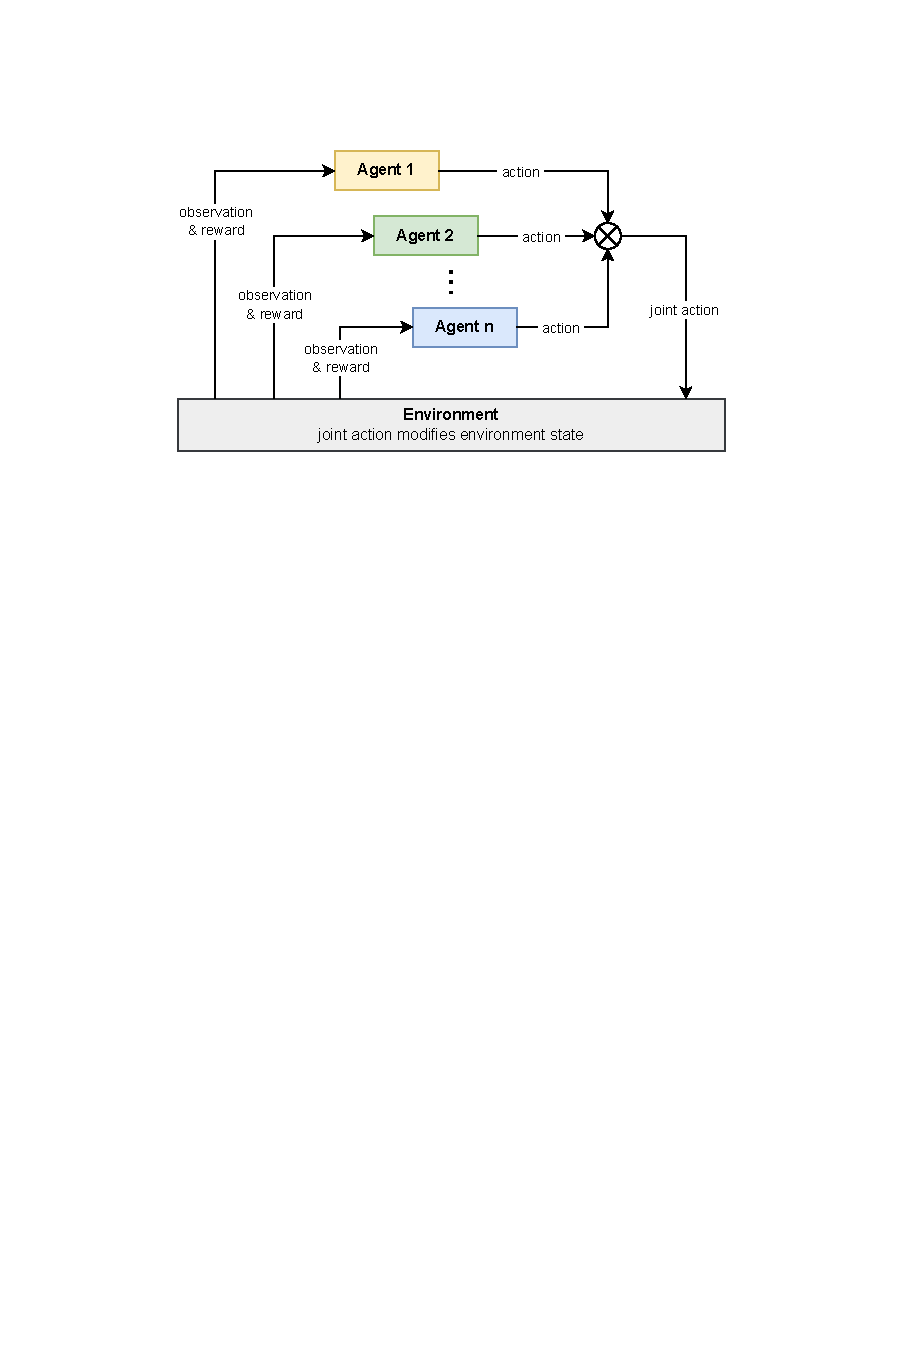
\includegraphics[width=0.7\linewidth]{assets/2/rl_multi_agent_schematic.pdf}
    \caption[Schematica dell'Apprendimento per Rinforzo multi-agente]{Schematica dell'Apprendimento per Rinforzo multi-agente, in cui un insieme di n agenti ricevono delle osservazioni individuali sullo stato dell'ambiente, e scelgono delle azioni per modificare lo stato. Ogni agente quindi riceve una ricompensa numerica e una nuova osservazione. Fonte: \cite{Stefano2024}}
    \label{fig:2_rl_multi_agent_schematic}
\end{figure}

\paragraph{Fasi di addestramento ed esecuzione.} In MARL la distinzione tra fase di addestramento e di esecuzione ha particolare importanza, perché permette di categorizzare gli approcci principali, approfonditi in \cite{Stefano2024}:

\begin{itemize}
    \item Addestramento ed esecuzione centralizzata: le due fasi avvengono in modo centralizzato, condividendo le informazioni disponibili su tutti gli agenti. Questo è l'approccio migliore per ottenere una buona coordinazione tra agenti, ma non tutti i problemi ammettono tale configurazione. Infatti, richiede di condividere le osservazioni e le decisioni, non sempre consentito per vincoli di privacy o comunque complesso in ambienti decentralizzati. 

    \item Addestramento ed esecuzione decentralizzata: non c'è una condivisione delle informazioni tra agenti in nessuna fase, ogni agente impara ed esegue azioni solo in base alle proprie osservazioni. Un importante limite di questo approccio è che l'ambiente non è più stazionario, violando pertanto la proprietà di Markov: le transizioni e la ricompensa non dipendono più soltanto dallo stato corrente. 

    \item Addestramento centralizzato, esecuzione decentralizzata: mira a equilibrare i due metodi, assumendo che sia possibile centralizzare l'addestramento (per esempio con una simulazione) mentre l'esecuzione avviene in modo completamente decentralizzato.
\end{itemize}

\paragraph{Cooperazione o collaborazione.} In uno scenario MARL gli agenti possono avere interessi diversi tra loro: si figurano dunque scenari competitivi, in cui gli interessi degli agenti sono contrapposti, scenari collaborativi, in cui gli interessi sono gli stessi, o scenari misti.

\subsection{Approccio Deep Learning}

Il Deep Reinforcement Learning (DRL) rappresenta un ramo dell'apprendimento per rinforzo che fonde il RL e il Deep Learning. Algoritmi di questa tipologia utilizzano le reti neurali per l'addestramento dell'agente, approssimando le funzioni di valore $V^\pi$ o $Q^\pi$, le politiche $\pi$ o il modello $P$.

Rispetto all'apprendimento supervisionato, nel DRL l'input e l'output per le reti neurali non sono fornite in anticipo, bensì i dati sono ottenuti dall'interazione tra l'agente e l'ambiente. La generazione dei dati e la valutazione dei risultati presenta inoltre difficoltà aggiuntive, poiché la funzione che la rete neurale impara è strettamente legata all'MDP: lo scambio di dati tra l'agente e l'ambiente è interattivo e limitato, inoltre l'esperienza raccolta viola l'assunzione per la discesa del gradiente, cioè che i dati siano distribuiti in modo identico e indipendente.

Nonostante le difficoltà sopracitate, il DRL ha guadagnato popolarità negli ultimi anni perché algoritmi di questa tipologia sono in grado di ottenere ottimi risultati in ambienti con ampi spazi delle azioni e delle osservazioni, e con dinamiche complesse. Diversi esperimenti hanno dimostrato un livello di capacità paragonabile se non superiore all'essere umano, dai videogiochi ad applicazioni reali della robotica e guida autonoma \cite{Mnih2015, Silver2017, Levine2016, Pan2017}.

In \Cref{fig:2_rl_algorithm_taxonomy} è mostrata una tassonomia dei principali algoritmi di RL e DRL moderni, caratterizzati per tipologia di funzione su cui si basano.

\begin{figure}
    \centering
    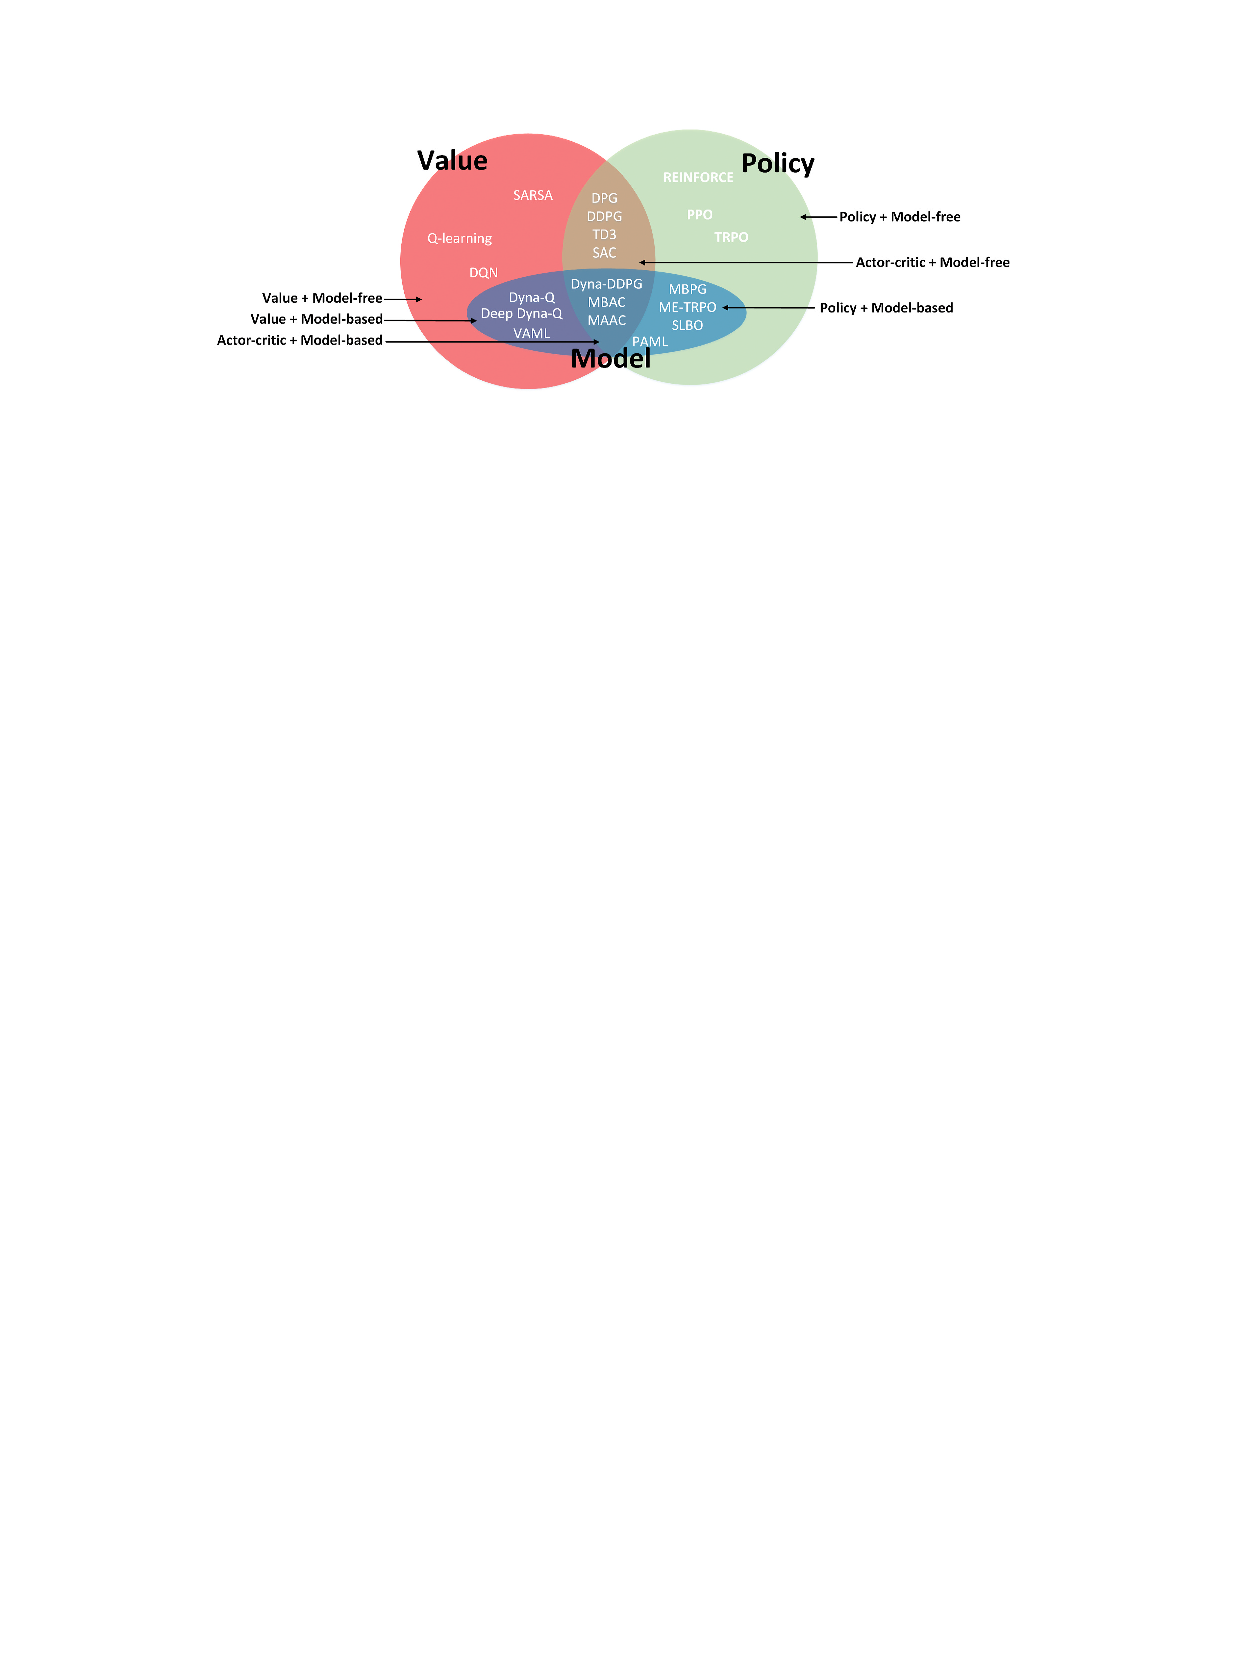
\includegraphics[width=\linewidth]{assets/2/rl_algorithm_taxonomy.pdf}
    \caption[Tassonomia dei principali algoritmi di RL e DRL moderni]{Tassonomia  dei principali algoritmi di RL e DRL moderni. Fonte: \cite{Perera2021}}
    \label{fig:2_rl_algorithm_taxonomy}
\end{figure}

\subsubsection{Metodi policy-gradient}

In DRL una policy viene rappresentata come una rete neurale con dei parametri $\theta$. Ogni insieme di valori $\theta$ rappresenta una particolare policy e l'addestramento dell'agente consiste nel trovare un insieme di valori $\theta$ che produce una policy ottimale.

I metodi policy-gradient hanno l'obiettivo di ottimizzare le prestazioni dell'agente trovando una policy $\pi_\theta$ in grado di generare una traiettoria $\tau$ che massimizza la ricompensa attesa, invece di apprendere una funzione di valore.

La funzione obiettivo nei metodi policy-gradient consiste nel massimizzare $J(\theta)$, ossia il valore atteso scontato per ottenere una policy $\pi_\theta$ aggiornando i parametri $\theta$:

\begin{equation}
    J(\pi_\theta) = \mathbb{E}_{\tau \sim \pi_\theta} \left[ \sum_{t=0}^{T} \gamma^t r_t\right],
\end{equation}

\begin{equation}
    \theta^\ast = \underset{\theta}{\arg\max} \, J(\pi_\theta).
\end{equation}

Si utilizza l'ascesa del gradiente stocastica per aggiornare i parametri $\theta$ in direzione positiva del gradiente della misura di prestazioni della policy $\nabla_\theta J(\theta)$, tramite la seguente equazione

\begin{equation}
    \theta \gets \theta + \alpha \nabla_\theta J(\pi_\theta),
\end{equation}

in cui $\alpha$ è uno scalare che regola il tasso di apprendimento.

Il vantaggio principale degli approcci policy-gradient risiede nella stabilità della loro convergenza: questi metodi funzionano aggiornando direttamente la loro policy a ogni passo, invece di aggiornare la funzione di valore da cui derivare la policy come nei metodi value-based. Quest'ultimi possono portare a un cambio radicale nell'output della policy anche per un piccolo cambio nella funzione di valore, causando oscillazioni prominenti durante l’addestramento. Inoltre, gli algoritmi policy-gradient possono affrontare spazi di azione continui poiché l’agente stima direttamente l’azione invece di calcolare il valore per ogni azione discreta possibile. La terza caratteristica è la loro capacità di apprendere policy stocastiche, utili in contesti incerti o ambienti parzialmente osservabili. Nonostante i vantaggi sopra menzionati, i metodi policy-gradient hanno uno svantaggio sostanziale: tendono a convergere verso un massimo locale invece che il massimo globale.

\paragraph{Architettura Actor-Critic.} Risulta naturale combinare due o più funzioni fondamentali, introdotte nella \Cref{sec:2_rl_algorithms_types}, per realizzare algoritmi che ottengano il meglio di ognuno. Un insieme di questi algoritmi sono quelli che imparano una policy e una funzione di valore, chiamati ``Actor-Critic''. Sono chiamati in questo modo perché la policy agisce, mentre la funzione di valore critica.

In DRL, ci sono due reti neurali: una che decide l'azione da intraprendere, chiamata ``Actor'', e una che valuta le azioni compiute dalla rete Actor, chiamata ``Critic''. Quest'ultima rete viene utilizzata per calcolare l'errore di previsione del valore, che è la differenza tra il valore stimato e il guadagno atteso, poi usato per aggiornare le due reti neurali.

L'idea alla base è che durante l'addestramento la funzione di valore può fornire più informazioni per la policy rispetto alla sequenza di ricompense date dall'interazione con l'ambiente. La policy impara a utilizzare le informazioni fornite dalla funzione di valore e le usa per generare azioni. L'algoritmo presentato e utilizzato nel seguente studio è di questa tipologia.

\subsection{Proximal Policy Optimization}
\label{sec:2_ppo}

Proximal Policy Optimization (PPO), introdotto in \cite{Schulman2017}, è un algoritmo di DRL di tipo policy-gradient, model-free che alterna il campionamento dei dati, tramite l'interazione con l'ambiente, con l'ottimizzazione di una funzione obiettivo surrogata utilizzando l'ascesa del gradiente stocastica. Ha una struttura Actor-Critic, pertanto impara la policy ottimale tramite la rete actor, e la funzione di valore tramite la rete critic, per cui è value-based. Inoltre PPO è policy-based poiché la rete actor impara la policy tramite metodi policy-gradient.

Un problema presente negli algoritmi policy-gradient è che sono suscettibili al collasso delle prestazioni, in cui un agente comincia ad agire male. Questo scenario è difficile da recuperare, poiché l'agente comincia a generare traiettorie poco utili per addestrare la policy. Inoltre un problema presente negli algoritmi on-policy è che non possono riutilizzare l'esperienza raccolta. PPO affronta questi due problemi introducendo una funzione obiettivo surrogata, la quale evita il collasso delle prestazioni garantendo dei miglioramenti monotonici per la policy. Tale obiettivo inoltre permette di riusare esperienza off-policy per la fase di addestramento.

\paragraph{Versioni di PPO.} PPO basa la sua ottimizzazione sul concetto di trust-region, ovvero l’introduzione di un vincolo tra gli aggiornamenti della policy, al fine di non avere cambiamenti troppo bruschi nell'aggiornamento della policy. Per fare ciò, PPO utilizza due euristiche: la prima basata sull'uso della penalità adattiva KL, la seconda basata sull'obiettivo surrogato clipped. Le due euristiche sono semplici da implementare ed efficaci; nell'articolo originale la versione con l'obiettivo surrogato clipped ha ottenuto prestazioni migliori rispetto all'altra, tuttavia le implementazioni disponibili in librerie pubblicamente accessibili forniscono abitualmente entrambe.

\subsubsection{Vantaggio} Nel contesto del RL e in particolare nei metodi basati su policy-gradient come PPO gioca un ruolo importante il concetto di vantaggio. Denotato con $A_t$, il vantaggio è una misura che quantifica quanto meglio, o peggio, sia eseguire una certa azione $a_t$ in uno stato $s_t$ rispetto al valore medio delle azioni in quello stato secondo la policy corrente. Può essere espresso come

\begin{equation}
    A_t = Q_t(s_t, a_t) - V_t(s_t)
\end{equation}

in cui $Q_t$ è la funzione azione-valore, rappresentante il guadagno atteso per l'azione $a_t$ dallo stato $s_t$, e $V_t$ è la funzione di valore, rappresentante il guadagno atteso medio dallo stato $s_t$, entrambe in base alla policy attuale $\pi$.

In PPO, il vantaggio è utilizzato per ponderare gli aggiornamenti della policy durante il processo di apprendimento. Se un’azione ha prodotto un vantaggio positivo significa che ha prodotto un guadagno superiore alla media e, di conseguenza, la probabilità di scegliere tale azione in futuro dovrebbe essere incrementata. Al contrario, se il vantaggio è negativo la probabilità di scegliere tale azione dovrebbe essere ridotta.

\subsubsection{Funzione obiettivo surrogata} PPO usa il concetto di massimizzazione della funzione obiettivo surrogata:

\begin{align}
    L^{\textnormal{CPI}}(\theta) &\coloneqq \mathbb{E}_t \left[ \frac{\pi_\theta(a_t | s_t)}{{\pi_\theta}_\textnormal{old}(a_t | s_t)} {A_t}^{{\pi_\theta}_\textnormal{old}} \right] \label{eq:2_ppo_surrogate_objective_full} \\
    &\coloneqq \mathbb{E}_t \left[ r_t(\theta) A_t \right], \label{eq:2_ppo_surrogate_objective}
\end{align}

in cui $\frac{\pi_\theta(a_t | s_t)}{{\pi_\theta}_\textnormal{old}(a_t | s_t)}$ rappresenta una stima della divergenza tra le due policy successive ${\pi_\theta}$ e ${\pi_\theta}_\textnormal{old}$, mentre ${A_t}^{{\pi_\theta}_\textnormal{old}}$ è il vantaggio calcolato con la vecchia policy.

Per semplicità di notazione si userà l'\Cref{eq:2_ppo_surrogate_objective}, che è equivalente all'\Cref{eq:2_ppo_surrogate_objective_full} con la differenza che $r_t(\theta) = \frac{\pi_\theta(a_t | s_t)}{{\pi_\theta}_\textnormal{old}(a_t | s_t)}$ e $A_t = {A_t}^{{\pi_\theta}_\textnormal{old}}$.

L'obiettivo è quello di valutare e migliorare la prestazioni della nuova policy $\pi_\theta$ rispetto alla vecchia ${\pi_\theta}_\textnormal{old}$. $L^{\textnormal{CPI}}(\theta)$ come funzione obiettivo è stata proposta inizialmente in \cite{Kakade2002}.

\subsubsection{Funzione obiettivo surrogata clipped}
\label{sec:2_ppo_funzione_obiettivo_clipped}

Senza un vincolo, la massimizzazione di $L^{\textnormal{CPI}}$ produrrebbe degli aggiornamenti alla policy troppo ampi che porterebbero a un collasso delle prestazioni. Per questo motivo $L^{\textnormal{CPI}}$ viene modificata penalizzando i cambiamenti di policy che rendono $r_t(\theta)$ eccessivamente lontano da 1:

\begin{equation}
    L^{\textnormal{CLIP}}(\theta) \coloneqq \mathbb{E}_t \left[ \min \left (r_t(\theta) A_t, \textnormal{clip}(r_t(\theta), 1 - \epsilon, 1 + \epsilon) A_t \right ) \right].
\end{equation}

$L^{\textnormal{CLIP}}$ è la funzione obiettivo surrogata clipped, in cui $\epsilon$ è un iperparametro che determina il grado di variazione ammesso per la policy in ogni aggiornamento, per evitare aggiornamento troppo bruschi che potrebbero destabilizzare l'apprendimento.

Notare che il primo termine di $\min$ è $L^{\textnormal{CPI}}$. Il termine $\textnormal{clip}(r_t(\theta), 1 - \epsilon, 1 + \epsilon)$ rimuove l'incentivo di muovere $r_t$ al di fuori dell'intervallo $[1 - \epsilon, 1 + \epsilon]$.

La funzione $L^{\textnormal{CLIP}}$ calcola quindi il valore minimo tra i due termini indicati, allo scopo di impedire variazioni troppo significative della policy, proteggendo il processo di apprendimento da possibili instabilità e oscillazioni.

La \Cref{fig:2_ppo_clip} mostra il funzionamento di $L^{\textnormal{CLIP}}$ in un singolo passo $t$.

\begin{figure}
    \centering
    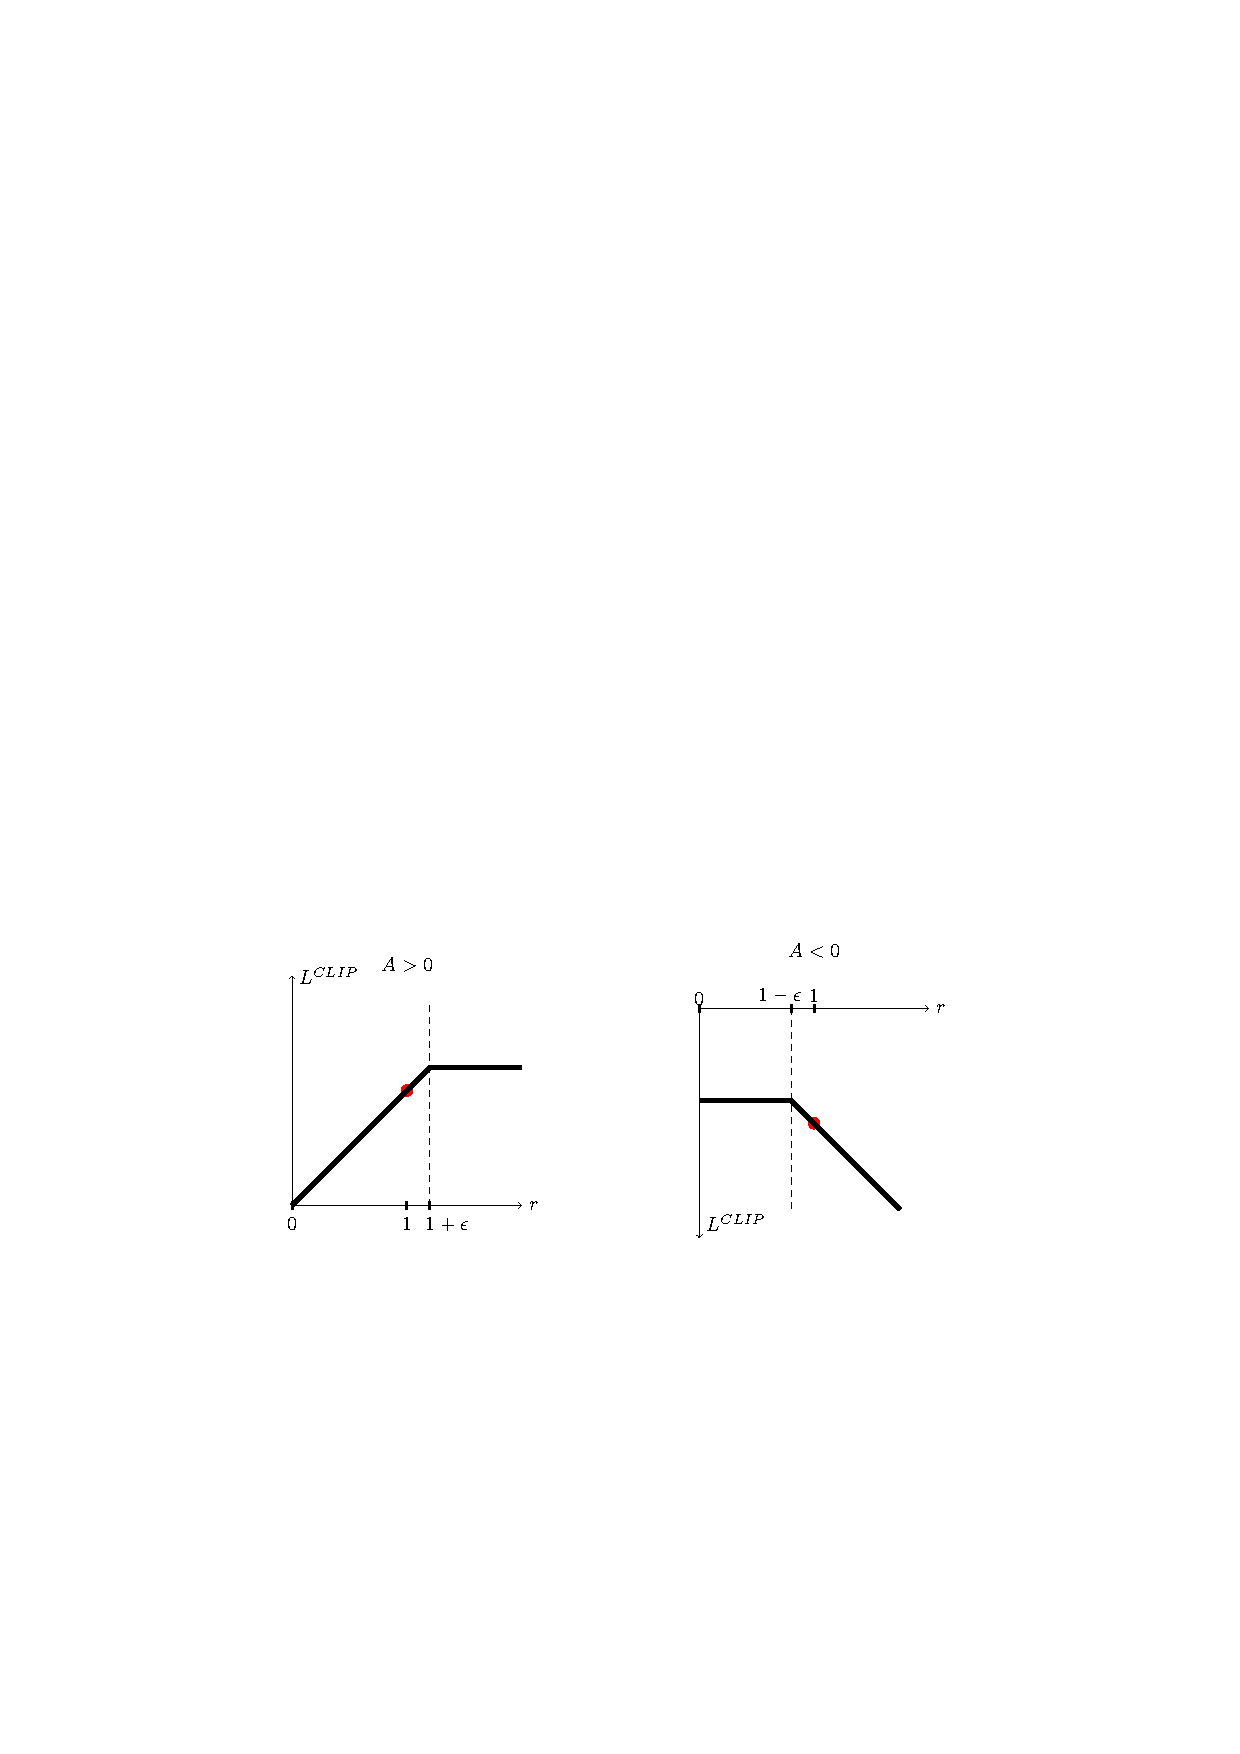
\includegraphics[width=.7\linewidth]{assets/2/ppo_clip.pdf}
    \caption[Esempio di funzionamento di $L^{\textnormal{CLIP}}(\theta)$]{Esempio di funzionamento di $L^{\textnormal{CLIP}}(\theta)$ come funzione del rapporto di probabilità $r$. A sinistra il caso di un vantaggio positivo, a destra un vantaggio negativo. In rosso è rappresentato il punto iniziale di ottimizzazione (in questo esempio $r = 1$. Fonte: \cite{Schulman2017}}
    \label{fig:2_ppo_clip}
\end{figure}
    
\subsubsection{Penaltà KL adattiva}

Un'alternativa alla funzione obiettivo surrogata clipped, applicabile separatamente oppure in aggiunta, è di utilizzare una penalità basata sulla divergenza di Kullback–Leibler\footnote{Una misura non simmetrica della differenza tra due distribuzioni di probabilità.} (KL), e di adattare un coefficiente di penalità in base al problema. $L^{\textnormal{CPI}}$ viene quindi modificata nel modo seguente:

\begin{equation}
    L^{\textnormal{KLPEN}}(\theta) \coloneqq \mathbb{E}_t \left[ r_t(\theta) A_t - \beta \, \textnormal{KL}[{\pi_\theta}_\textnormal{old}(\cdot | s_t), \pi_\theta(\cdot, s_t)] \right].
\end{equation}

$L^{\textnormal{KLPEN}}$ è la funzione obiettivo surrogata KL-penalizzata, in cui $\beta$ è un coefficiente adattivo che controlla la dimensione della penalità KL. $\beta$ è aggiornato a ogni aggiornamento della policy e il nuovo valore viene utilizzato nella successiva iterazione. L'aggiornamento si basa sulla comparazione di un iperparametro $d_\textnormal{targ}$ e dal valore $d = \mathbb{E}_t \left[ \textnormal{KL}[{\pi_\theta}_\textnormal{old}(\cdot | s_t), \pi_\theta(\cdot, s_t)] \right]$:

\begin{itemize}
    \item Se $d < d_\textnormal{targ} / 1.5$, allora $\beta \gets \beta / 2$,
    \item Se $d > d_\textnormal{targ} \times 1.5$, allora $\beta \gets \beta \times 2$.
\end{itemize}

Il valore iniziale dell'iperparametro $\beta$ non è rilevante perché l'algoritmo lo corregge automaticamente, mentre i parametri costanti $1.5$ e $2$ sono state scelte euristicamente in \cite{Schulman2017}, ma l'algoritmo non è particolarmente sensibile a tali valori.

\subsubsection{L'algoritmo}

Come già introdotto, PPO adotta un'architettura Actor-Critic. Questa architettura permette di formulare una funzione obiettivo che integra l'ottimizzazione delle due reti neurali, incorporando sia la differenza tra i valori previsti dalla rete Critic e il guadagno effettivo, sia la differenza tra le azioni scelte dalla rete Actor e quelle ottimali.

Inoltre si aggiunge un bonus di entropia $S$, che serve a incoraggiare una maggiore esplorazione da parte della rete Actor, prevenendo la convergenza prematura verso una policy deterministica. La funzione obiettivo risultante, in base alla scelta di usare $L^{\textnormal{CLIP}}$ o $L^{\textnormal{KLPEN}}$ (o entrambi), massimizzata a ogni iterazione è la seguente:

\begin{equation}
    L^{\textnormal{CLIP+VF+S}}_t(\theta) \coloneqq \mathbb{E}_t \left[ L^{\textnormal{CLIP}}_t(\theta) - c_1 L^{\textnormal{VF}}_t + c_2 S[\pi_\theta](s_t) \right]
\end{equation}

in cui $c_1$ e $c_2$ sono dei coefficienti, $S$ è il bonus di entropia e $L^{\textnormal{VF}}_t$ è l'errore quadratico $(V_\theta(s_t) - V^{\textnormal{targ}}_t)^2$.

PPO esegue la policy per un numero di passi $T$, un numero minore della lunghezza totale dell'episodio, in modo da ottenere più minibatch (insieme di esperienza) da ogni episodio. Ciò consente di realizzare aggiornamenti frequenti e informativi della policy, senza necessità di completare interi episodi.

L'algoritmo è mostrato in \Cref{alg:2_ppo} come pseudocodice. Nella sua versione originale, sono presenti $N$ attori che eseguono contemporenamente la policy ${\pi_\theta}_\textnormal{old}$ in diversi ambienti per $T$ passi, raccogliendo l'esperienza raccolta come forma di traiettorie. L'ottimizzazione viene effettuata con l'esperienza raccolta tramite SDG (discesa del gradiente stocastica) in minibatch, ognuno di dimensione $M$.

\begin{algorithm}
    \caption[Pseudocodice di Proximal Policy Optimization (PPO)]{Pseudocodice di Proximal Policy Optimization (PPO)}
    \label{alg:2_ppo}
    \begin{algorithmic}[1] % Every line gets a number.
        \For{iterazione = 1, 2, ...}
            \For{attore = 1, 2, ..., $N$}
                \State Esegui la policy ${\pi_\theta}_\textnormal{old}$ nell'ambiente per $T$ passi;
                \State Calcola le stime dei vantaggi $A_1, \dots, A_t$ usando ${\pi_\theta}_\textnormal{old}$;
            \EndFor
            \State Ottimizza $L(\theta)$, per $K$ epoche e con la dimensione dei minibatch $M \le NT$;
            \State $\theta_\textnormal{old} \gets \theta$;
        \EndFor
    \end{algorithmic}
\end{algorithm}

Il calcolo dei vantaggi è definito come

\begin{equation}\label{eq:2_ppo_advantages}
    A_t = \delta_t + (\gamma \lambda) \delta_{t+1} + \dots + (\gamma \lambda)^{T-t+1} \delta_{T-1},
\end{equation}

in cui $\delta_t = r_t + \gamma V(s_{t+1}) - V(s_t)$ e $t$ è un indice temporale in $[0, T]$. L'\Cref{eq:2_ppo_advantages} è una versione troncata della stima del vantaggio generalizzata (GAE), introdotta in \cite{Schulman2015}.

\subsection{Scelte per il caso di studio}
\label{sec:2_rl_ppo_choices}

Nella modellazione del problema DFaaS, approfondita nella \Cref{sec:4_environments}, è stato scelto uno spazio di azione continuo per indicare quali richieste sono da processare localmente, inoltrare e rifiutare. Questo ha condizionato la scelta dell'algoritmo, perché non tutti sono compatibili con tale spazio. PPO è un algoritmo che supporta gli spazi d'azione continui. Inoltre è facile da implementare e non richiede troppe risorse computazionali. Rispetto ad altri algoritmi simili come Soft Actor-Critic (SAC), ha dimostrato prestazioni migliori in problemi simili a quello affrontato \cite{Haarnoja2018, Petriglia2024}.

Nel considerare la modellazione multi-agente, sono stati sperimentati due approcci principali di MARL con PPO:

\begin{itemize}
    \item Fase di addestramento ed esecuzione decentralizzata: in cui ogni agente ha una policy indipendente dalle altre, imparata con le osservazioni locali dell'agente. In termini pratici, significa utilizzare PPO per ogni agente.

    \item Fase di addestramento centralizzata ed esecuzione decentralizzata: nella fase di addestramento PPO viene eseguiti in modo centralizzato condividendo i parametri della rete Critic per tutti gli agenti, mentre la rete Action, quella che apprende la policy, rimane indipendente. Nella fase di esecuzione ogni agente ottiene una copia della rete Critic addestrata ed esegue la policy senza la condivisione delle informazioni.
\end{itemize}